\documentclass[12pt,preprint]{aastex6}
\usepackage{amsmath,amssymb}
\usepackage{graphicx}
\usepackage{float}
\usepackage{multirow}
\usepackage{threeparttable}
\usepackage{appendix}
\usepackage{longtable}
\usepackage{color}
\usepackage{tikz}






\begin{document}

\title{Tests on IMCOM: Generating NIRCam Mosaics}

\author{Sara Crandall and Brant Robertson}

\affil{Department of Astronomy \& Astrophysics, University of California Santa Cruz\\ 
                 211 Interdisciplinary Sciences Building\\
                  Santa Cruz, CA 95064, USA} 
\email{sacranda@ucsc.edu, brant@ucsc.edu}

\section*{}
\begin{center}
This document logs the steps taken to generate mosaic mock images for NIRCam use.
\end{center}




\maketitle
\section{An introduction to IMCOM}
IMage COMbination (IMCOM) may be a useful tool for generating mosaic mock images for NIRCam. This software was designed by \cite{Rowe2011} for use on WFIRST, and it allows undersampled images to be combined into an oversampled image. This would be useful for NIRCam, as some bands provide undersampled images. DRIZZLE is commonly used for image combination, but may have resolution loss resulting from reduced control of the PSF in the combined image. The Fourier/linear algebra technique is also useful, but can be less reliable when positions are not well known. A least-squares tool is beneficial in that output noise can be minimized. IMCOM uses a combination of these three methods to reconstruct an image with a controlled PSF, knowing the positions of exposures, that also minimizes noise. 

To ensure that IMCOM is the right tool for NIRCam use, we will run a few tests. As described in the software's documentation, a baseline set of arguments are required. The command line looks like
\begin{equation}
\label{imcom_input}
\mathrm{./imcom \ <config{\_}file>  \ <U/S> \ <U/S{\_}max> \ <U/S{\_}tol>}.
\end{equation}
Here, the input $\mathrm{<U/S>}$ will either minimize the leakage objective, $U_\alpha$, (the local leakage or difference between the desired PSF and the reconstruction) or the noise covariance for each output pixel, $\Sigma_{\alpha\alpha}$. $\mathrm{<U/S{\_}max>}$ defines the maximum leakage objective or noise covariance, $U_{\alpha}^{\mathrm{max}}$ and $\Sigma_{\alpha\alpha}^{\mathrm{max}}$ respectively, depending on the previous option. $\mathrm{<U/S{\_}tol>}$ defines $\Delta U_{\alpha}^{\mathrm{tol}}$ or $\Delta\Sigma_{\alpha\alpha}^{\mathrm{tol}}$ that specify when the iteration should stop. The program will finish when $U_{\alpha}^{\mathrm{max}}-\Delta U_{\alpha}^{\mathrm{max}}<U_{\alpha}\leq U_{\alpha}^{\mathrm{max}}$ or $\Sigma_{\alpha\alpha}^{\mathrm{max}}-\Delta \Sigma_{\alpha\alpha}^{\mathrm{max}}<\Sigma_{\alpha\alpha}\leq \Sigma_{\alpha\alpha}^{\mathrm{max}}$. 







\section{Test${\_}0$}
Test${\_}$0 will determine which IMCOM inputs are useful for our purposes by varying the above options.\footnote{There are other inputs that can be specified such as the convolution and objective kernels, designated as ``soft inputs" in \cite{Rowe2011}, but they won't be varied at the moment.} IMCOM has two examples included with the package (userxy0 and userxy1) which we will use those for our initial tests. Userxy1 gives the user more freedom to designate the input pixel locations.

To begin, example userxy0 will be used and the U/S option will be varied. The following inputs were used:
\begin{equation}
\mathrm{config{\_}example\ U\ 1.d-3\ 1.d-6}\footnote{Double precision floating point numbers are used}
\end{equation}
and
\begin{equation}
\mathrm{config{\_}example \ S \ 1.d-3 \ 1.d-6}.
\end{equation} 
The results are seen in Figure \ref{fig:varyUandS} along with an ideal output provided with the IMCOM package. Residuals between the ideal and ``U" \& ``S" options are also shown. All three residuals are near zero. 

%%%%%%Figure 1
%%%%%%%%%%
\begin{figure}[!htbp]
\centering
\advance\leftskip-1.0cm
\advance\rightskip-1.0cm
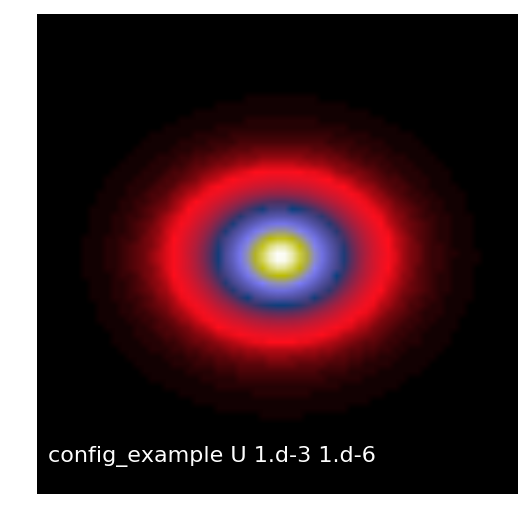
\includegraphics[height=60mm,width=60mm]{f1a.png}
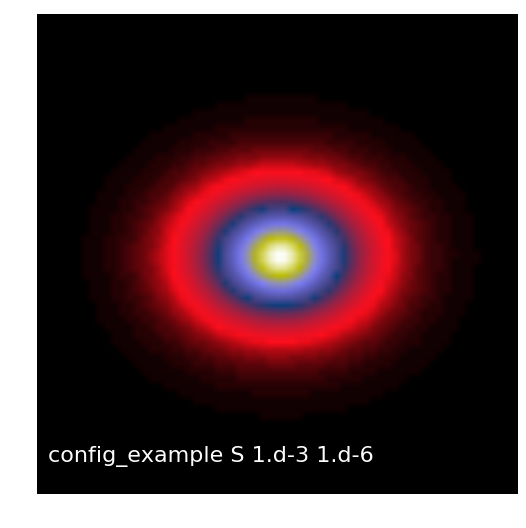
\includegraphics[height=60mm,width=60mm]{f1b.png}
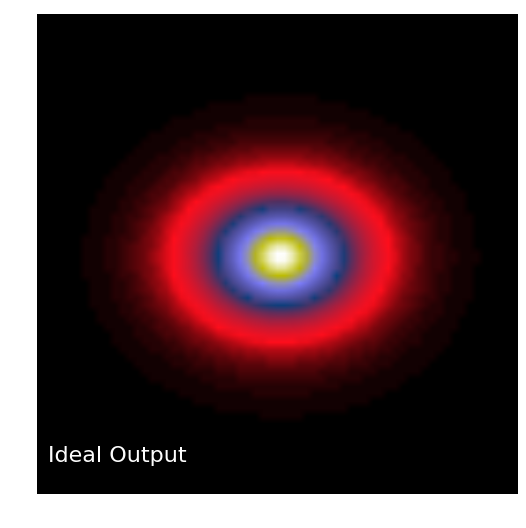
\includegraphics[height=60mm,width=60mm]{f1c.png}
\raisebox{0.045\height}{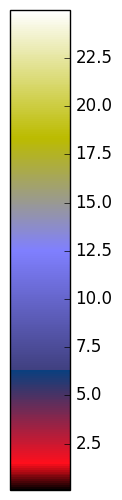
\includegraphics[height=57mm,width=15mm]{f1d.png}}
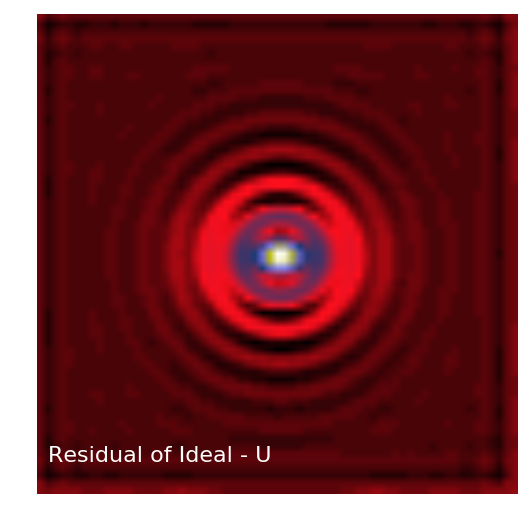
\includegraphics[height=60mm,width=60mm]{f1e.png}
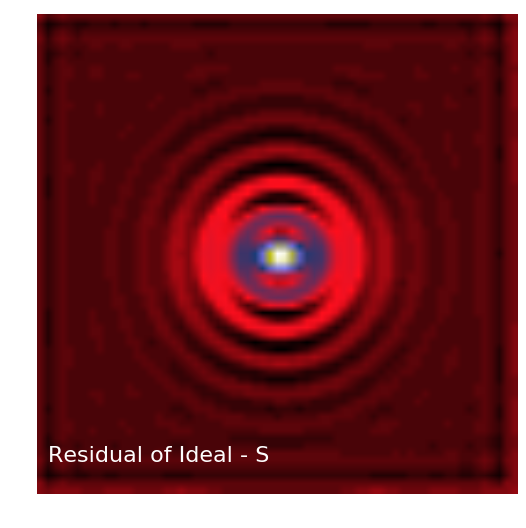
\includegraphics[height=60mm,width=60mm]{f1f.png}
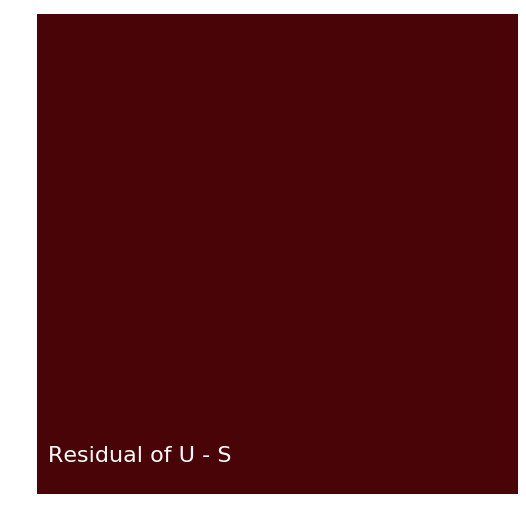
\includegraphics[height=60mm,width=60mm]{f1g.png}
\raisebox{0.045\height}{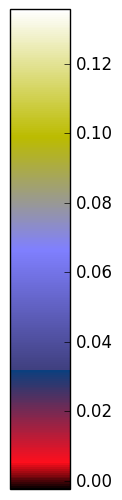
\includegraphics[height=57mm,width=15mm]{f1h.png}}
\caption{The top-left and top-center images use the ``$U$" and ``$S$" options, respectively. The top-right image is the ideal output included with IMCOM. The bottom row shows residuals that are near zero.}
\label{fig:varyUandS}
\end{figure}

Next, the userxy0/userxy1 option will be varied. The input
\begin{equation}
\mathrm{config{\_}example \ U \ 1.d-3 \ 1.d-6}
\end{equation}
is used. Figure \ref{fig:varyxy0andxy1} shows the results, including the residuals from the ideal output minus the IMCOM output.
%%%%%%Figure 2
%%%%%%%%%%
\begin{figure}[!htbp]
\centering
\advance\leftskip-1.0cm
\advance\rightskip-1.0cm
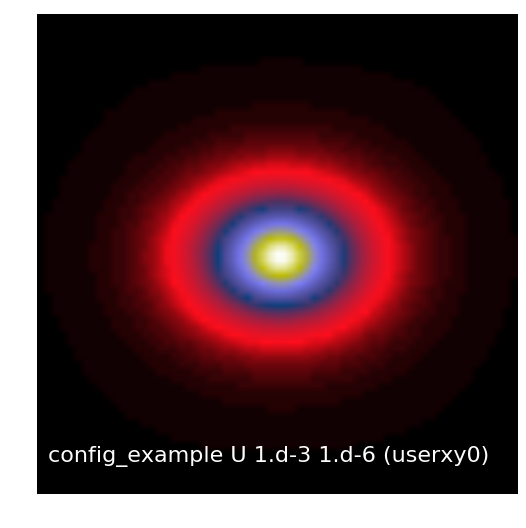
\includegraphics[height=45mm,width=45mm]{f2a.png}
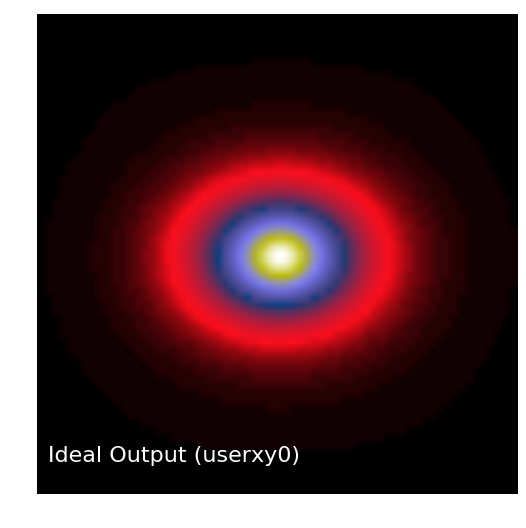
\includegraphics[height=45mm,width=45mm]{f2b.png}
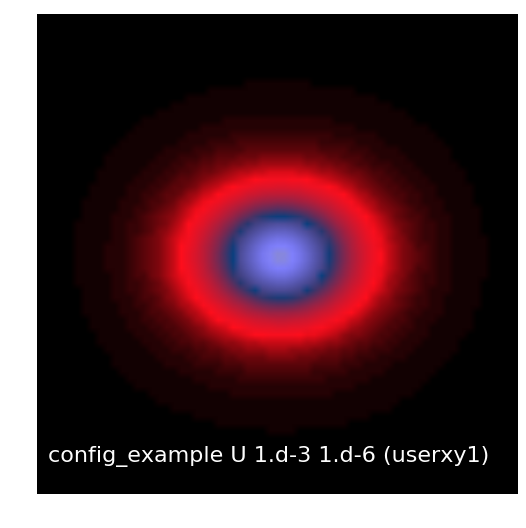
\includegraphics[height=45mm,width=45mm]{f2c.png}
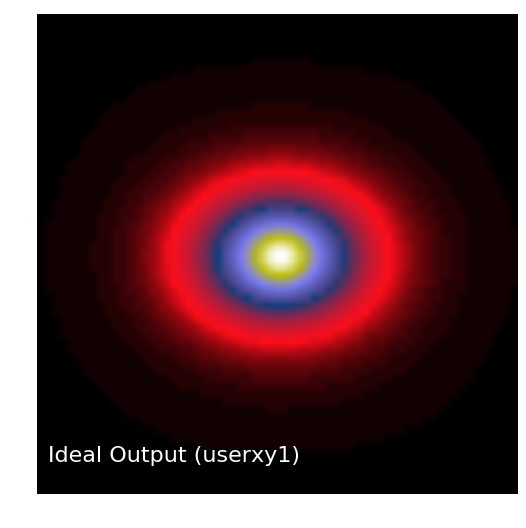
\includegraphics[height=45mm,width=45mm]{f2d.png}
\raisebox{0.045\height}{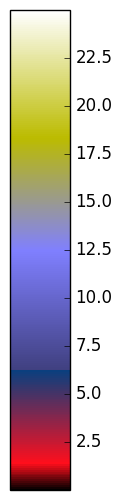
\includegraphics[height=42.5mm,width=10mm]{f2e.png}}
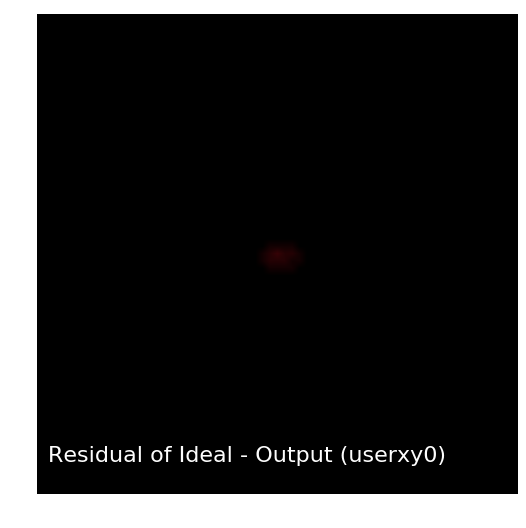
\includegraphics[height=60mm,width=60mm]{f2f.png}
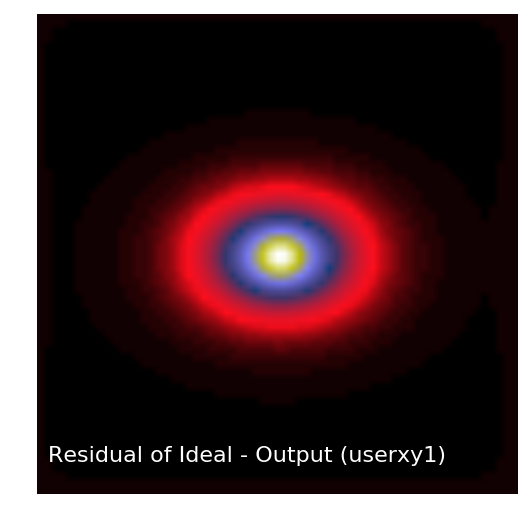
\includegraphics[height=60mm,width=60mm]{f2g.png}
\raisebox{0.035\height}{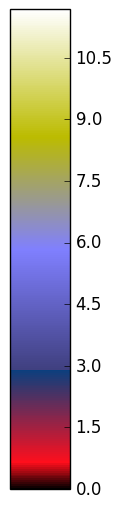
\includegraphics[height=57.5mm,width=15mm]{f2h.png}}
\caption{The top images use the userxy0 example with the left, center, and right panels being the IMCOM output, ideal output, and residual respectively. The bottom images use the userxy1 example with the left, center, and right panels being the IMCOM output, ideal output, and residual respectively.}
\label{fig:varyxy0andxy1}
\end{figure}
The userxy1 option is less defined and has a larger residual. This may not be surprising as the userxy1 option allows a user input for pixel centering, and may result in a more realistic output image.









\section{Test${\_}$1}
We will move forward with using the userxy1 example, as the pixel locations need to be provided. We will also focus on minimizing the leakage objective, as we are concerned with how well the output image matches the inputs.\footnote{Minimizing U${\_}$tol can result in a reconstruction that is not trustworthy, as the algorithm may not reach an ideal reconstruction.} With these options in mind we will vary U${\_}$max and U${\_}$tol, and call this exercise ``Test${\_}$1." U${\_}$max and U${\_}$tol were varied from 1.d-1 to 1.d-10, as IMCOM gives warning messages for smaller values. Figure \ref{fig:vary_umax_utol} shows several examples of this test along with the residuals of the ideal minus the output images. We see that smaller values as well as small differences in U${\_}$max and U${\_}$tol result in smaller residuals between the output and ideal images. 
%%%%%%Figure 3
%%%%%%%%%%  
\begin{figure}[!htbp]
\centering
\advance\leftskip-1.0cm
\advance\rightskip-1.0cm
\hspace{3.5cm}
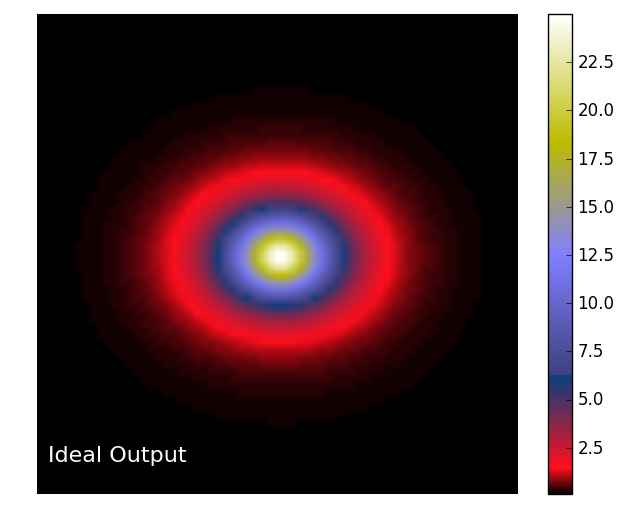
\includegraphics[height=50mm,width=50mm]{f3a.png}
\newline
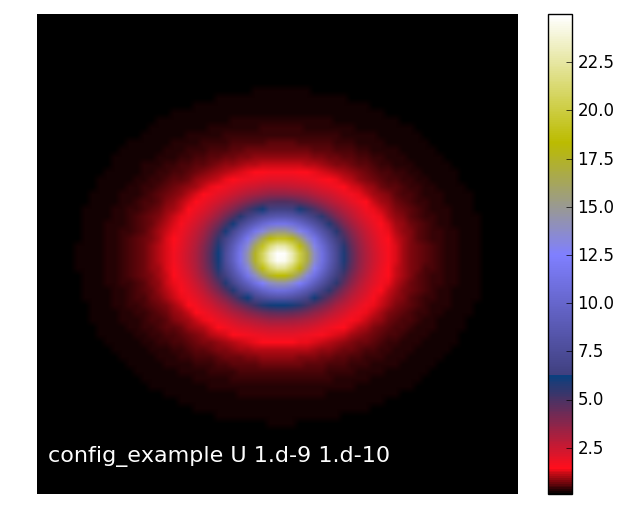
\includegraphics[height=47mm,width=49mm]{f3b.png}
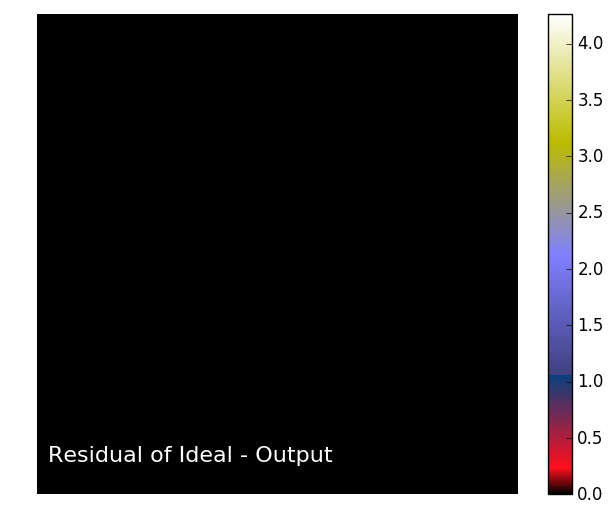
\includegraphics[height=47mm,width=49mm]{f3c.png}
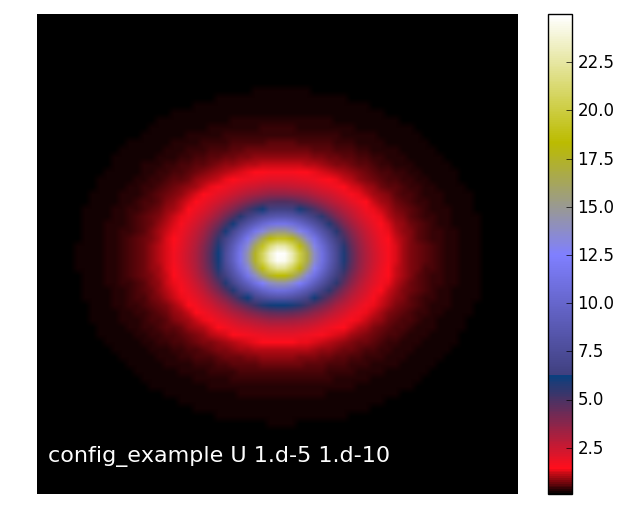
\includegraphics[height=47mm,width=49mm]{f3d.png}
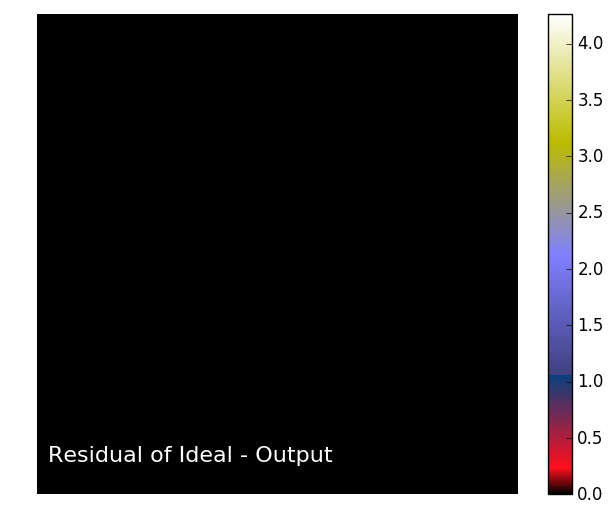
\includegraphics[height=47mm,width=49mm]{f3e.png}
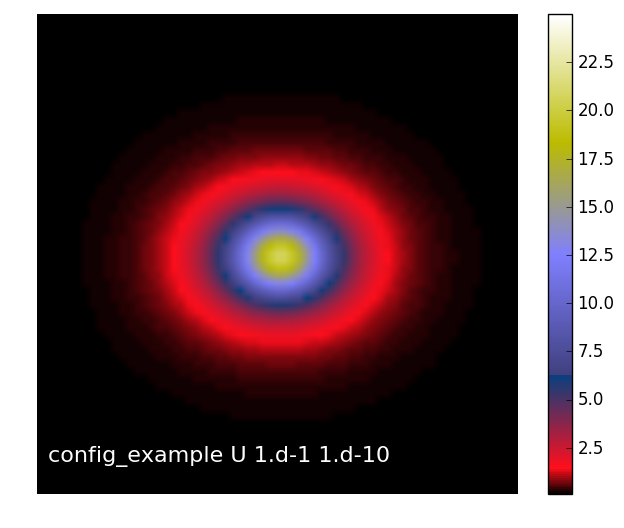
\includegraphics[height=47mm,width=49mm]{f3f.png}
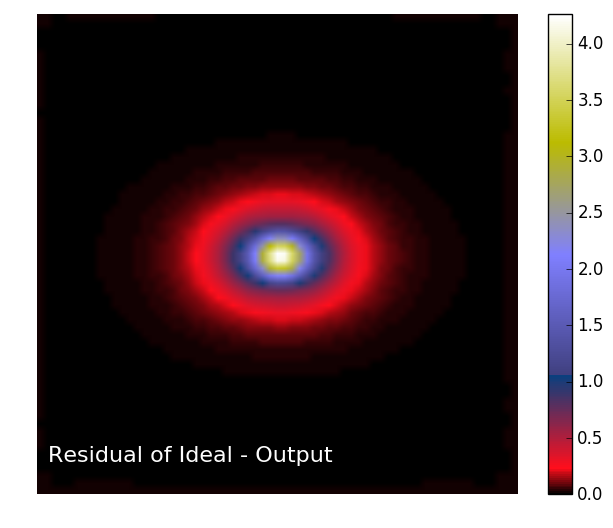
\includegraphics[height=47mm,width=49mm]{f3g.png}
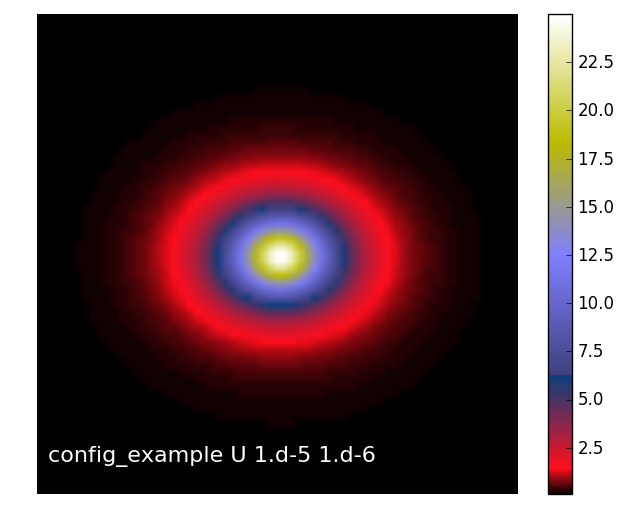
\includegraphics[height=47mm,width=49mm]{f3h.png}
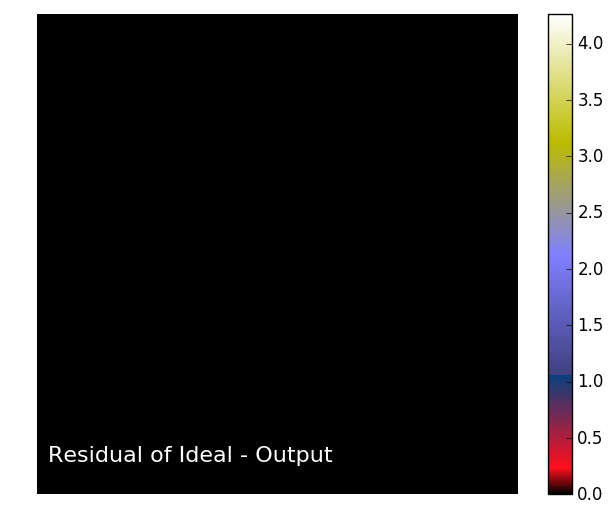
\includegraphics[height=47mm,width=49mm]{f3i.png}
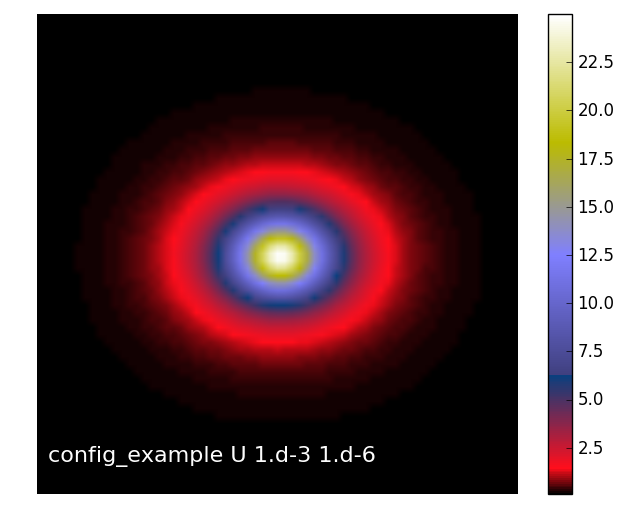
\includegraphics[height=47mm,width=49mm]{f3j.png}
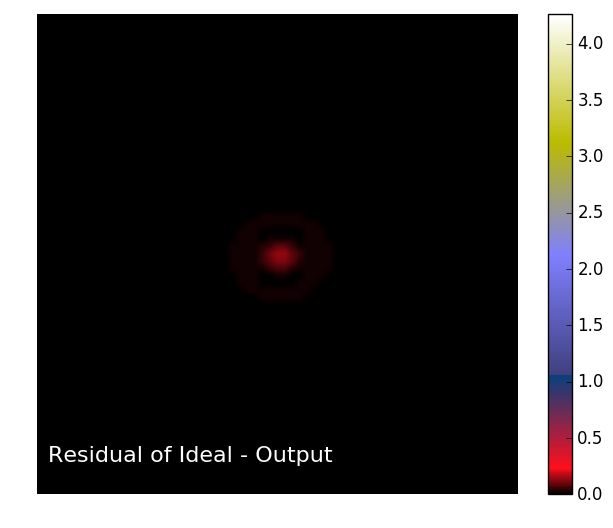
\includegraphics[height=47mm,width=49mm]{f3k.png}
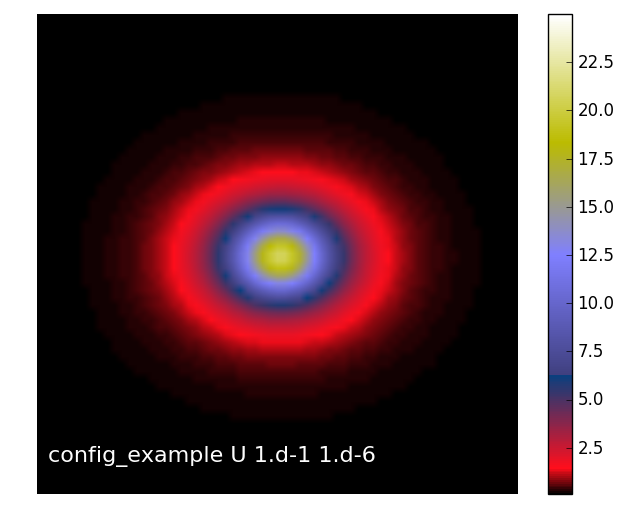
\includegraphics[height=47mm,width=49mm]{f3l.png}
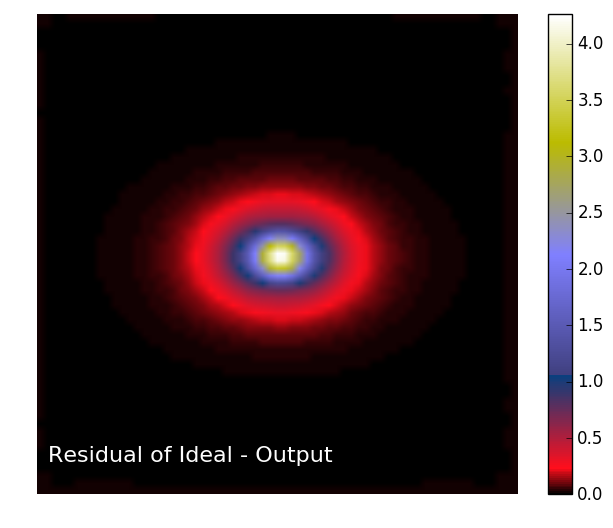
\includegraphics[height=47mm,width=49mm]{f3m.png}
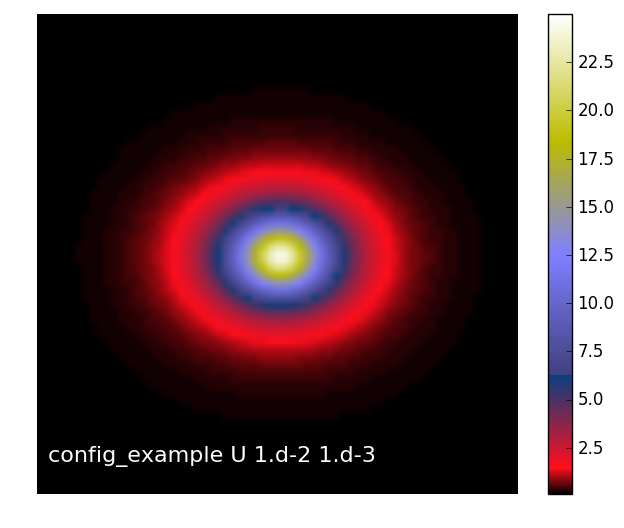
\includegraphics[height=47mm,width=49mm]{f3n.png}
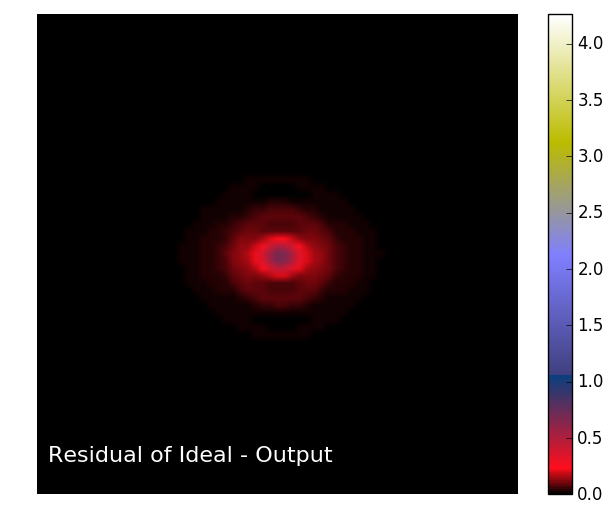
\includegraphics[height=47mm,width=49mm]{f3o.png}
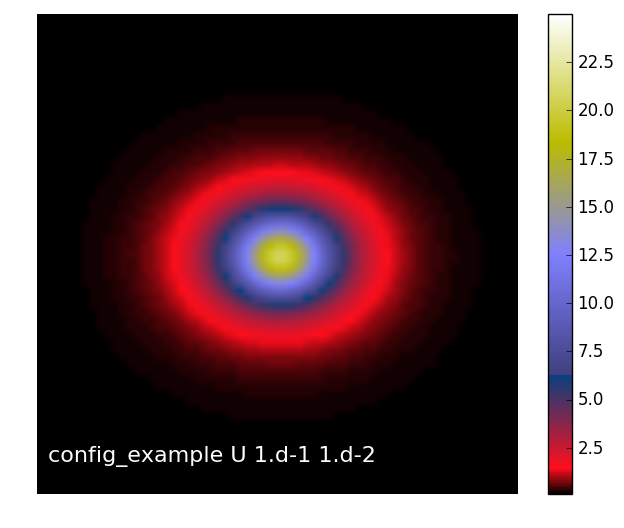
\includegraphics[height=47mm,width=49mm]{f3p.png}
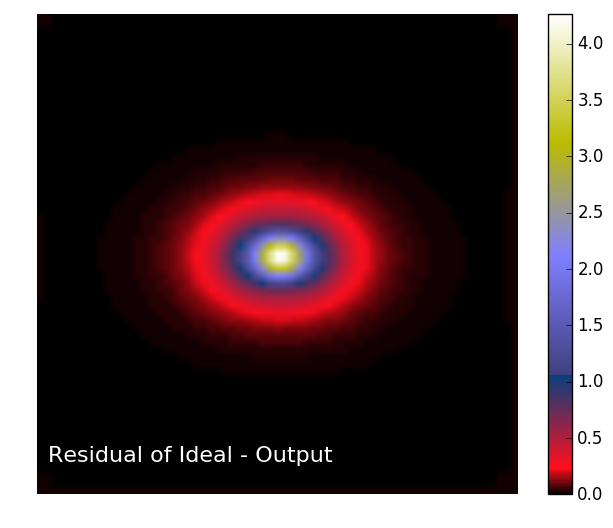
\includegraphics[height=47mm,width=49mm]{f3q.png}
\caption{Output images using userxy1 example, U option, and varying U${\_}$max \& U${\_}$tol.}
\label{fig:vary_umax_utol}
\end{figure}
  




\section{Test${\_}$2}
We now move on to ``Test${\_}$2," where we see how well IMCOM can handle noise in the input images. First, we will use small U${\_}$max and U${\_}$tol inputs to decrease the differences in output and ideal output images (as demonstrated in Test${\_}$1). We use the IMCOM input
\begin{equation}
\mathrm{config{\_}example \ U \ 1.d-9 \ 1.d-10}
\end{equation}
for the userxy1 example. The overall goal here is to investigate how the differences in the IMCOM output and ideal images are affected by the signal to noise ratio ($S/N$). 


To add noise, we draw random values from a Poisson distribution given by
\begin{equation}
P(k)=\frac{\lambda^{k}e^{-\lambda}}{k!},
\label{Eq:poisson}
\end{equation}
and add to existing input images. Here $\lambda$ depends on the $S/N$, which we will vary. That is
\begin{equation}
\lambda=\left(\frac{<S_{p}>}{S/N}\right)^2,
\label{Eq:lambda}
\end{equation}
where $<S_{p}>$ is the average signal from the input images given by
\begin{equation}
<S_{p}>=\frac{\sum_{i}p_{i}\Delta A_{i}}{\sum_{i}\Delta A_{i}}.
\label{Eq:avg_sig}
\end{equation}
Here, $p_{i}$ is the pixel and $\Delta A_{i}$ is the area of the pixel. 

We generate noisy images for $0<S/N\leq15$ in increments of 0.25. Figure \ref{fig:noise} shows the input exposures, IMCOM output, ideal, residual images for $S/N=5$ as an example. 
%%%%%%Figure 4
%%%%%%%%%%
\begin{figure}[!htbp]
\centering
\advance\leftskip-1.0cm
\advance\rightskip-1.0cm
%\hspace{3.5cm}
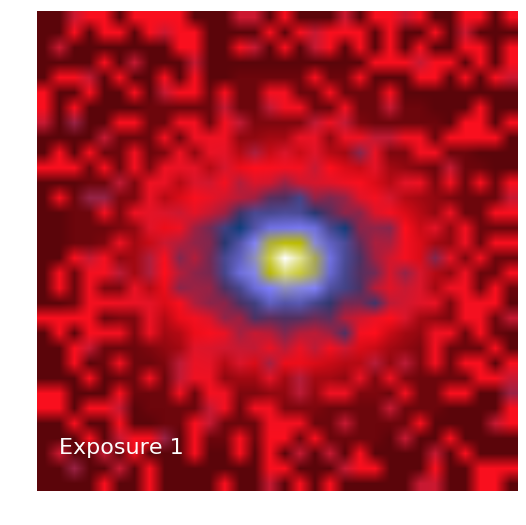
\includegraphics[height=45mm,width=45mm]{f4a.png}
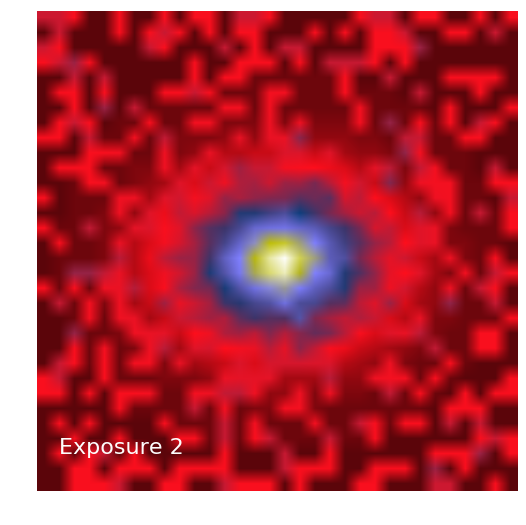
\includegraphics[height=45mm,width=45mm]{f4b.png}
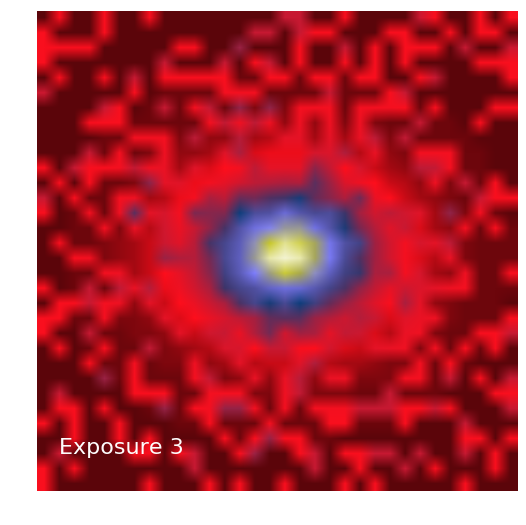
\includegraphics[height=45mm,width=45mm]{f4c.png}
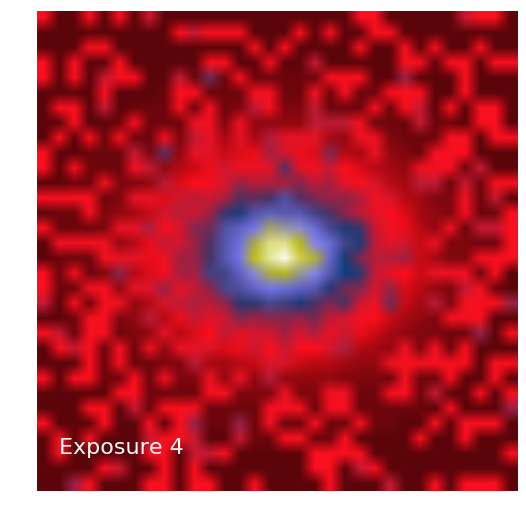
\includegraphics[height=45mm,width=45mm]{f4d.png}
\raisebox{0.045\height}{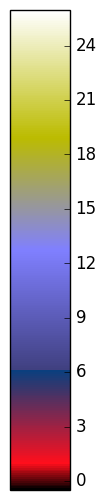
\includegraphics[height=43mm,width=11mm]{f4e.png}}
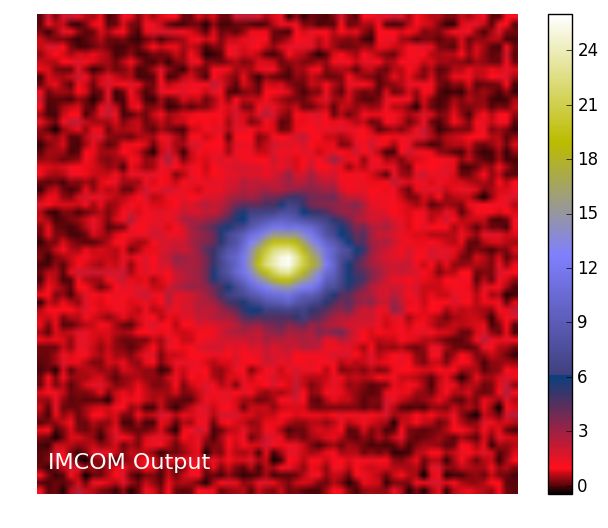
\includegraphics[height=60mm,width=60mm]{f4f.png}
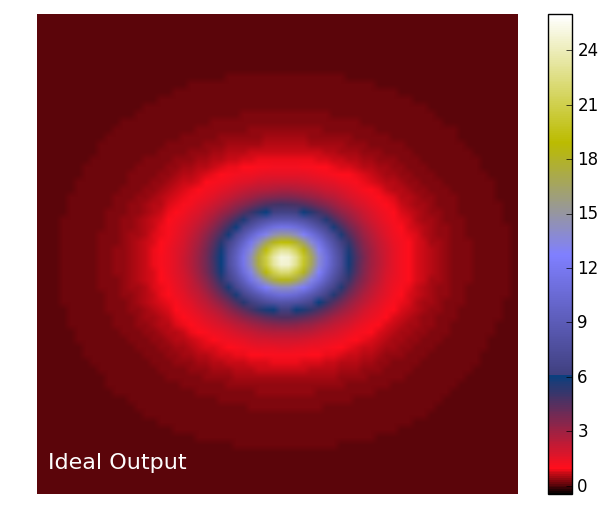
\includegraphics[height=60mm,width=60mm]{f4g.png}
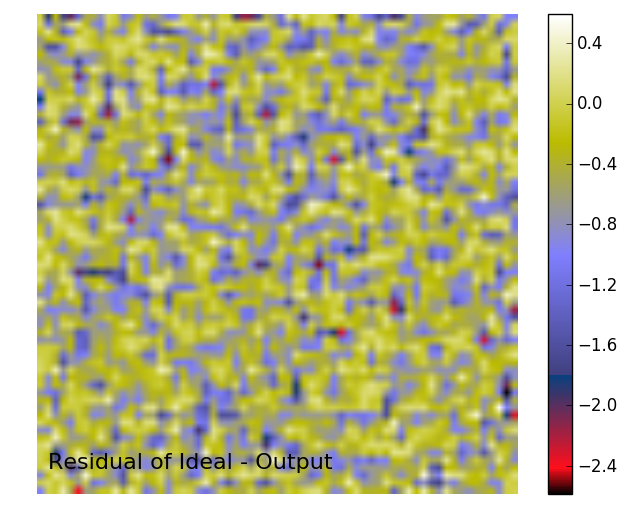
\includegraphics[height=60mm,width=60mm]{f4h.png}
\caption{Noise added to input images for the $S/N=5$ case.}
\label{fig:noise}
\end{figure}


We further explore how IMCOM handles noise by combining images one exposure at a time (see Figure \ref{fig:noise_by_exp}). However, the output of combing only two exposures is quite poor, and so by putting each combination output on the same scale, the images are washed out????

%%%%%%Figure 5
%%%%%%%%%%
\begin{figure}[!htbp]
\centering
\advance\leftskip-1.0cm
\advance\rightskip-1.0cm
\hspace{3.5cm}
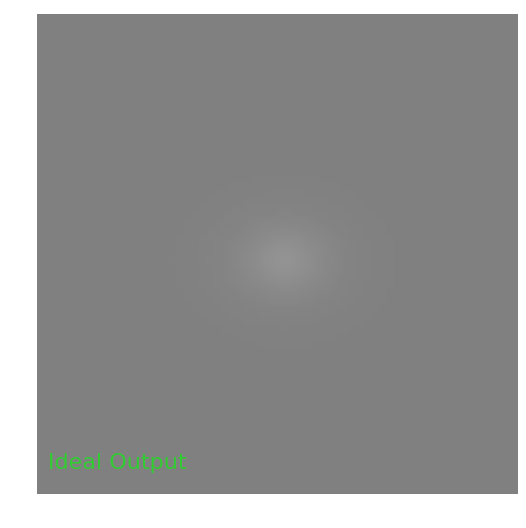
\includegraphics[height=60mm,width=60mm]{f5a.png}
\newline
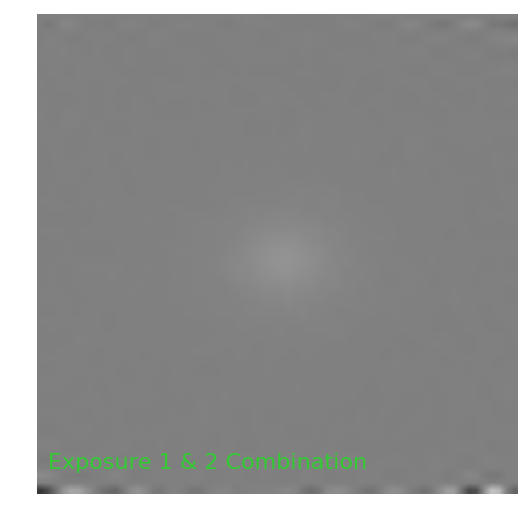
\includegraphics[height=60mm,width=60mm]{f5b.png}
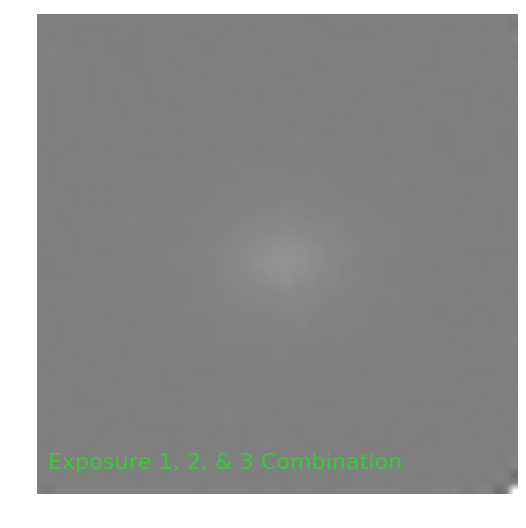
\includegraphics[height=60mm,width=60mm]{f5c.png}
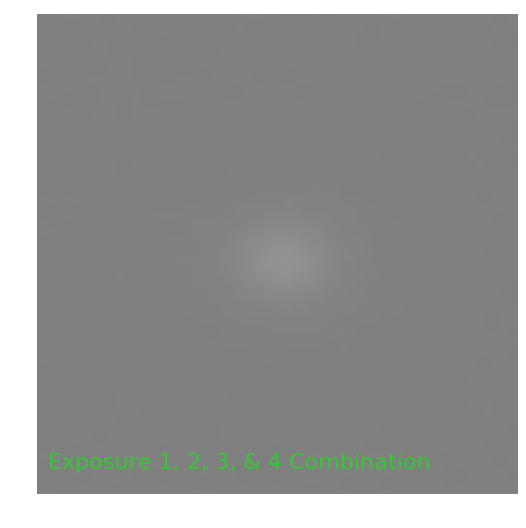
\includegraphics[height=60mm,width=60mm]{f5d.png}
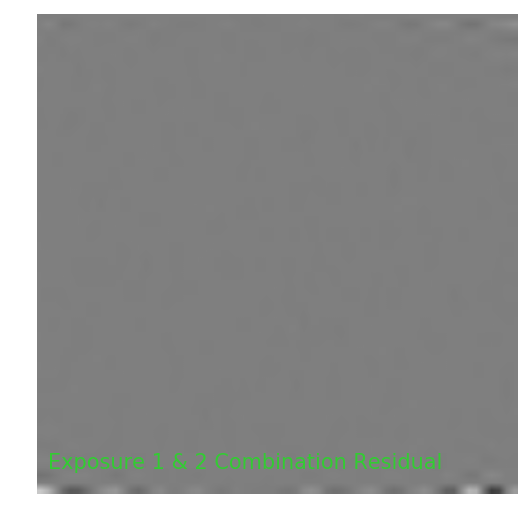
\includegraphics[height=60mm,width=60mm]{f5e.png}
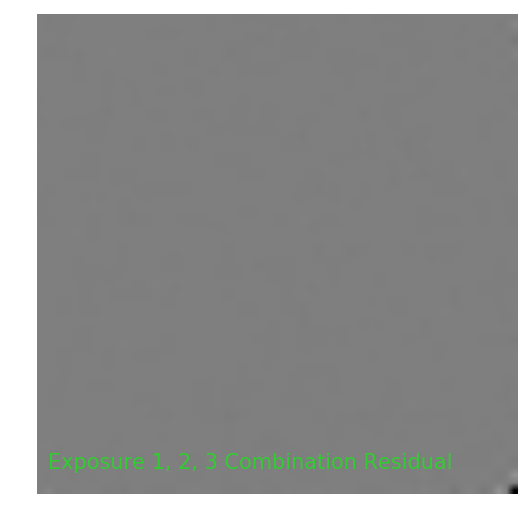
\includegraphics[height=60mm,width=60mm]{f5f.png}
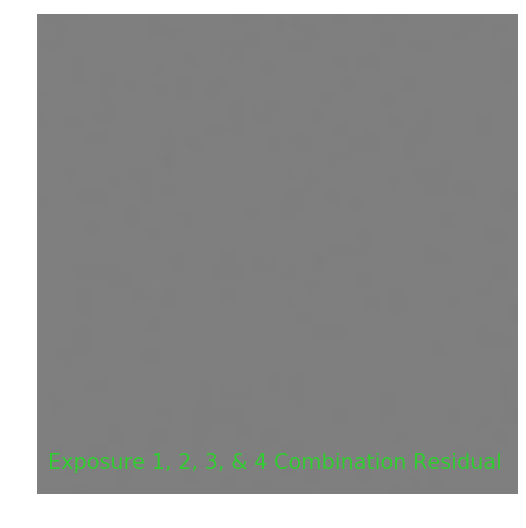
\includegraphics[height=60mm,width=60mm]{f5g.png}
\caption{Noise added to input images for the $S/N=5$ case. Each middle panel shows the image combination with increasing exposure number. The bottom panels show the residuals between the corresponding IMCOM outputs and the ideal image.}
\label{fig:noise_by_exp}
\end{figure}

To quantify how the noise is being handled by IMCOM, we can plot $\chi^{2}$ vs. $S/N$ (see Figure \ref{fig:L2_vs_SNR}). We define $\chi^{2}$ as
\begin{equation}
\chi^{2}=\frac{1}{N-1}\sum_{i}^{N}\frac{(H_{i}-I_{i})^{2}}{|H_{i}|},
\label{Eq:chi2}
\end{equation}
where $H$ \& $I$ are the output and ideal image for pixel $i=1,2,....,N$.
%%%%%%Figure6 
%%%%%%%%%%
\begin{figure}[!htbp]
\centering
\advance\leftskip-1.0cm
\advance\rightskip-1.0cm
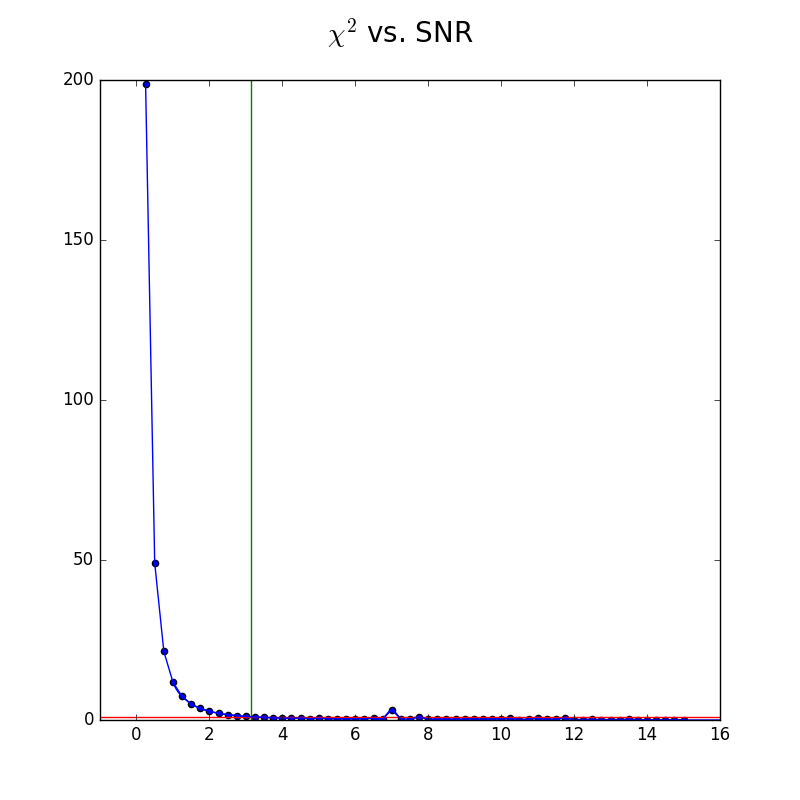
\includegraphics[height=65mm,width=65mm]{f6a.png}
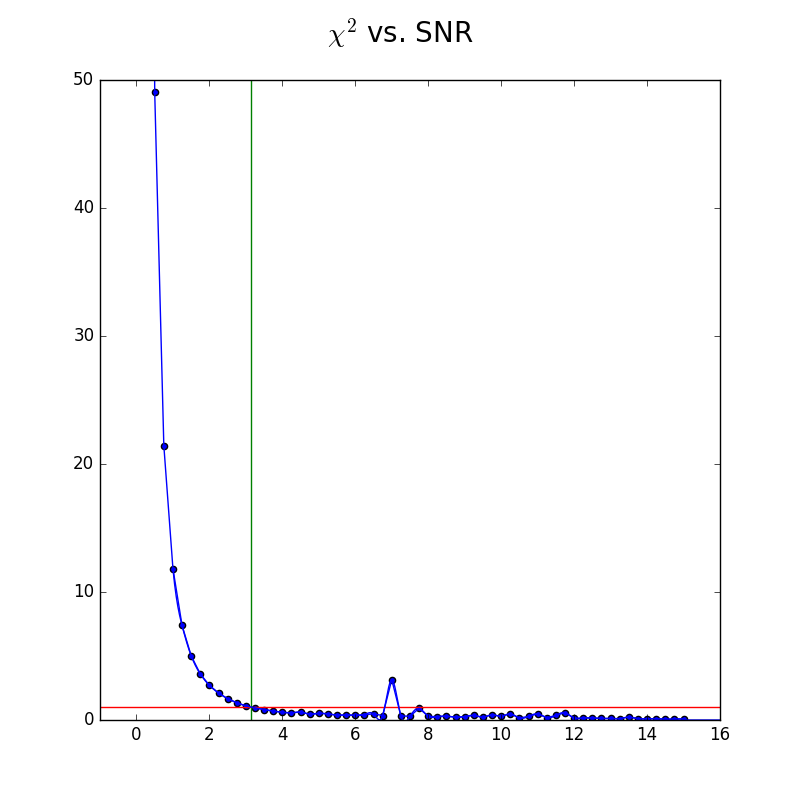
\includegraphics[height=65mm,width=65mm]{f6b.png}
\includegraphics[height=65mm,width=65mm]{f6c.png}
\caption{$\chi^{2}$ vs. $S/N$. for $S/N\leq15$. The center plot is a zoomed in version of the left, and the right plot shows a log of $\chi^{2}$ vs. $S/N$. The red line shows $\chi^{2}=1$ and the green line shows where $\chi^{2}$ intersects with 1.}
\label{fig:L2_vs_SNR}
\end{figure}
This plot is promising, as $\chi^{2}$ is reasonable for values $S/N>2$. There are deviations from the general trend around 7$<S/N<8$, but it is within normal expected error.






\newpage
\section{Test Conclusions}
Because IMCOM \citep[][]{Rowe2011} makes use of the benefits from common mosaicing tools, it is a ideal software package to generate JWST NIRCam mock mosaic images. It will be useful in that it gives control of the PSF in the combined image, minimizes noise, and is used by knowing the positions of the pixels. 

After running several tests on provided example images, it appears that IMCOM allows enough input freedom for the user. As an initial test, IMCOM can handle added noise to input images for at least $S/N>2$. 

In conclusion, IMCOM is a promising tool for NIRCam use, and we will continue to use it by testing mock images generated by Christopher Willmer.




\clearpage
\begin{thebibliography}{}

\def\apj{ApJ}

\bibitem[{{Rowe} {et~al.}(2011)}]{Rowe2011}
{Rowe}, B., {Hirata}, C., \& {Rhodes}, J. 2011, \apj, 741, 46

\end{thebibliography}


\end{document}